We want to extract \pcic sentences from \coq vernac (.v) files, in order to perform \premiseselection.
For this thesis we want to try various approaches to \premiseselection,
and we want to know how well our solution performs.
That is why we implemented the \premiseselection tool called \roerei.
Various design goals of this tool are to:
\begin{itemize}
    \item Support offline learning and analysis of \machinelearning on the various corpora.
    \item Enable integration in the \coqide GUI.
		We would like to create something like Clippy (see Figure \ref{figure:clippy}) or Vigor (see Figure \ref{figure:vigor}) for \coq.
		Both are integrated intelligent user interfaces that assist users using an interactive animated character.
    \item Enable merging of the premise selection tool in the \coq main branch as a plugin.
\end{itemize}
Ideally the tooling created can be used as a building block in a future \coq tactic which finishes proofs fully automatically.

\begin{center}
	\begin{minipage}{0.49\linewidth}
		\begin{figure}[H]
			\centering
			
\includegraphics[height=10em]{assets/clippy.png}
			\caption{Clippy for Microsoft Word}
			\label{figure:clippy}
		\end{figure}
	\end{minipage}
	\begin{minipage}{0.49\linewidth}
		\begin{figure}[H]
			\centering
			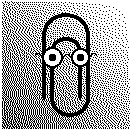
\includegraphics[height=10em]{assets/vigor.png}
			\caption{Vigor for VI}
			\label{figure:vigor}
		\end{figure}
	\end{minipage}
\end{center}

As we want \pcic sentences and not \gallina text, directly reading \coq vernac (.v) files will not be very useful.
During compilation of these vernac files \coq however generates \pcic terms internally.
These \pcic terms can be exported as so-called \acic terms using the \xml plugin distributed with \coq:
\begin{definition}[\acic]\defgls{acic}
	The Calculus of (Co)Inductive Constructions with Explicit Named Substitutions \cite{coen2000progettazione}.

	In normal \cic sections can contain local variables.
	After closing such a section, all definitions are discharged by abstracting these local section variables away.
	In \acic this is no longer necessary as the definitions are adapted to explicitly capture local variables.
\end{definition}

The tool is comprised of a \preloader and the main program \roerei.
The \preloader is implemented in \ocaml and handles importing the \xml generated by \coq and emitting summaries.
All other work, such as making predictions and measuring it's own performance is done by \roerei, which is implemented in \cpp.

The \machinelearning field favours \python and \matlab as the preferred development environments.
Thus we needed to re-implement various \machinelearning algorithms in \cpp.

\subsection{Transformations}
\label{section:transformations}
The premise selection tool works as follows, and can be summarised as in Figure \ref{figure:transformations}:
\begin{enumerate}
    \item Export all \coq objects from the standard library and the selected corpora to XML files during their compilation.
		\coq has an XML export functionality built in, until version 8.4pl5.
		Currently this is the only existing method to extract \coq objects.
		This process is more thoroughly described in Section \ref{section:extraction}.
	\item Read these objects from XML files back into canonical \acic\glsadd{acic} format in memory of the \preloader.
	\item From each \coqobj[s] of the form $\name[s] \objdef \term[s] : \type[s]$,
		yield a summary $<\name[s], \termset{s}, \typeset{s}>$.
		\begin{definition}[$\flatten{x}$]\defgls{flatten}
			For a given term (or type) $x$, yield the set of names referenced to in the term.
			\[ \flattensym : \terms \rightarrow 2^{\names} \]
		\end{definition}
		Given that definition, $\termset{s}$\glsadd{termset} is the set of names of all objects in the term $\term[s]$,
		and $\typeset{s}$\glsadd{typeset} is the set of all names in the type $\type[s]$.
		Note that other variants for this $\flatten{x}$ can be used.
    We can also extract the number of occurances of each name using $\countoccur{x}$\glsadd{countoccur}:
    \begin{definition}[$\countoccur{x}$]\defgls{countoccur}
			For a given term (or type) $x$, yield the number of times names are referenced in the term.
      \[ \countoccursym : \terms \rightarrow \mathbb{N}^{\names} \]
    \end{definition}
    Similarly we can also extract the minimum depth for which each name occurs as $\depthoccur{x}$\glsadd{depthoccur}.
		\begin{figure}[H]
			\[
				\begin{array}{rcl}
					\typeset{\texttt{O}}, \typeset{\texttt{S}}, \typeset{\texttt{nat\_id}}, \typeset{\texttt{plus}} & = & \{ \texttt{nat} \}\\
					\typeset{\texttt{nat\_ind}} & = & \{ 0, \texttt{S} \} \\
					\typeset{\texttt{plus\_0\_r}} & = & \{ \texttt{nat}, \texttt{eq}, \texttt{plus}, 0 \} \\
					& & \\
					\termset{\texttt{nat\_id}} & = & \emptyset \\
					\termset{\texttt{plus\_0\_r}} & = & \{ \texttt{eq\_sym}, \texttt{nat\_ind}, \texttt{eq\_refl}, \texttt{f\_equal}, \texttt{S} \}
				\end{array}
			\]
			\caption{Summaries yielded for the natural number example in Figure \ref{figure:natexample}}
		\end{figure}
		These summaries are written to disk, and read again into memory of \roerei.
	\item Distinguish theorems from other definitions, which yields the features and dependencies.
		Ideally we would like to take all objects of sort \sortprop to be the theorems.
		However this does not work in all cases, specifically for the \corn dataset.
		In order to solve this we use a heuristic as defined by Kaliszyk et al.\ \cite{kaliszyk2014machine}.
		Where we consider $\objs$ to be the set of all \coq objects, we take
    \[
      \begin{array}{rcll}
        \defs & = & \bigcup_{s \in S} \typeset{s} & \text{(Definition \ref{def:defs})}\glsadd{defs} \\
        \thms & = & (\bigcup_{s \in S} \termset{s}) \setminus \defs & \text{(Definition \ref{def:thms})}\glsadd{thms}
      \end{array}
    \]
		This is more extensively explained in Section \ref{section:thmsdefs}.
		\begin{figure}[H]
			\[
				\begin{array}{rcl}
					\defs & = & \{ 0, \texttt{S}, \texttt{nat}, \texttt{eq}, \texttt{plus} \} \\
					\thms & = & \{ \texttt{eq\_sym}, \texttt{nat\_ind}, \texttt{eq\_refl}, \texttt{f\_equal} \}
				\end{array}
			\]
			\caption{$\defs$ and $\thms$ for the natural number example in Figure \ref{figure:natexample}}
		\end{figure}
    \item From the $\thms$ and $\defs$ generate a \dagraph of dependencies and feature vector for all \coq objects.
      See Section \ref{section:feats} and Sections \ref{section:deps}.
		\todo{dagraph dependencies} \todo{feature vector}
	\item These features and dependencies can now be used to predict by bundling them with a predictor, for example \knn.
		\todo{predictors}
\end{enumerate}

\todo{crossvalidation}
\todo{metrics}
\todo{corpora}
\todo{combine predictors}
\todo{more features}

\begin{figure}[H]
	\centering
	\begin{tikzpicture}[auto, node distance=2.5cm, main/.style={draw,align=center}]
		\node[main] (coq) {\coqobj[s]\\inside coq};
		\node[main] (xml) [below of=coq] {XML\\representation};
		\node[main] (term) [below of=xml] {\coqobj[s]\\$\name \objdef \term : \type$};
		\node[main] (summary) [below of=term] {Summary\\$<\name[s], \termset{s}, \typeset{s}>$};
		\node[main] (definitions) [below right=2cm and 0cm of summary] {Definitions\\$\defs$};
		\node[main] (theorems) [below left=2cm and 0cm of summary] {Theorems\\$\thms$};
    \node[main] (features) [below of=definitions] {Features\\of theorems\\$\features{}{s}$};
    \node[main] (dependencies) [below of=theorems] {Dependencies\\of theorems\\$\deps{s}$};
		\node[main] (predictor) [below=7.0cm of summary] {Predictor};

		\draw[->] (coq) edge node {(1) Coq XML export} (xml);
		\draw[->] (xml) edge node {(2) Parser} (term);
		\draw[->] (term) edge node {(3) Resolver} (summary);
		\draw[->] (summary) edge node [right] {(4) $\bigcup_{s \in S} \typeset{s}$} (definitions);
		\draw[->] (summary) edge node [left] {$\bigcup_{s \in S} \termset{s} \setminus \defs$ (4)} (theorems);
		\draw[dashed] (definitions) edge node {(4)} (theorems);
		\draw[->] (theorems) edge node {(5)} (dependencies);
		\draw[->] (definitions) edge node {(5)} (features);
		\draw[->] (features) edge node [left] {(6)} (predictor);
		\draw[->] (dependencies) edge node [right] {(6)} (predictor);
	\end{tikzpicture}
	\caption{Transformations performed by the \premiseselection tooling.}
	\label{figure:transformations}
\end{figure}


\subsection{Extraction}
\label{section:extraction}
During compilation of a \coq project the \xml plugin has the capability to emit \xml files containing \acic objects.
This plugin is shipped with \coq by default until version 8.4pl5.
For later versions there is currently no equivalent functionality available for \coq.
To instruct the plugin to emit \xml the following variables need to be set when calling \texttt{coqc} (for example via a Makefile):
\begin{center}
	\lstinline{COQ_XML=-xml COQ_XML_LIBRARY_ROOT=<dest>}
\end{center}

For some corpora it can be troublesome to have the compiler emit proper \xml.
We have developed several patches for the datasets used in this thesis.
For more information on the specific versions and patches used,
view Section \ref{section:corpora} and the \texttt{data} folder in the repository for this thesis.

From the parsed \xml files only the following \acic constructs are used:
\begin{description}
    \item[(Co)Inductive definitions]
        These definitions are composed of a name, a type, and a list of constructors.
        Each constructor also is composed of a name and a type.
		A (Co)Inductive definition also yields an induction principle (\texttt{ind}) and a recursion scheme (\texttt{rec}) as separate terms.
    \item[Constants (definitions / theorems / axioms)]
		The types and bodies (the body is equivalent to the \acic term) of constants are defined in separate \xml files.
		This separation is an optimization, as once defined the proofs (terms) of theorems are irrelevant.
		For \coq it is sufficient to only know the type of a theorem.
		For definitions the term is absolutely necessary, as the definitions needs to be substituted when applied.
		However, conceptually theorems and definitions become indistinguishable when exported (see Section \ref{section:thmsdefs}).
        Axioms only generate a type, as the term of an axiom is empty.
\end{description}

The following objects are not used, but could be useful in future work:
\begin{description}
    \item[Proof in progress]
		Consists of a name, a type, a body and a list of dependencies (also called subgoals).
        These dependencies still need to be satisfied to complete the proof.
    \item[Tactics application]
        On a higher level, tactics can be applied in order to form a proof.
        These higher level constructs are dependent on the proof engine.
        A proof consisting of tactics can thus become invalid given another \coq version.
        For premise selection these tactics can help solve proofs more quickly, because the proofs they form are smaller.
\end{description}

\coq also exports variables, but these are not used.
A variable consists of a name and a type, and becomes a parameter when a theory which uses the variable is applied.
Thusfar there is no use for these variables within this thesis.

\subsection{Theorems and definitions}
\label{section:thmsdefs}

For the sake of \premiseselection, we would like to categorize all \coqobjs as either theorems or definitions.
\begin{definition}[theorem]\glsadd{theorem}
    Theorems are \coqobjs that have been proved based on previously established \coqobjs.
    They logically follow from the defined axioms.
\end{definition}

\begin{definition}[definition]\glsadd{definition}
    Definitions are all \coqobjs that are not theorems.
    They are either simply constants or purely transformative operations on such constants
    and can merely assist in establishing new proofs.
\end{definition}

\coq is based on the Curry-Howard isomorphism.
This means that the statements of proofs (what is proven) are encoded in the type of the theorems.
Axioms are then defined as simple constants, and used in the term of a theorem to justify proofs.
Thus on a logical level there is no distinction between a definition and a theorem.
\coq tries to track this distinction by having the type of theorems be of sort \sortprop.
Ideally we would like to take all objects of sort \sortprop to be the theorems.
However this does not work in all cases, specifically for the \corn dataset.
In the case of \corn the propositions are of type \cprop, which is of sort \sorttype.
\todo{example-corn}

In order to solve this we use a heuristic as defined by Kaliszyk et al.\ \cite{kaliszyk2014machine}.
Where we consider $\objs$ to be the set of all \coqobjs,

\begin{definition}\defgls{defs}\label{def:defs}
  we take the definitions to be the names in the types of all \coqobjs
  \[ \defs = \bigcup_{s \in \objs} \typeset{s} \]
\end{definition}

\begin{definition}\defgls{thms}\label{def:thms}
  we take the theorems to be the names in the terms of all \coqobj, excluding all definitions
  \[ \thms = (\bigcup_{s \in \objs} \termset{s}) \setminus \defs \]
\end{definition}

This provides an adequate distinction for our purposes.

\subsection{Features}
\label{section:feats}

For \premiseselection we would like to suggest new theorems (premises) for open proof goals.
These premises are selected according to the type of the proof goal (the names of the constants in the proof goal).
Specifically we call the set of aspects which describe a proof goal the set of feature keys.

\begin{definition}\defgls{featurekeys}\label{def:featurekeys}
  The set of feature keys $\featurekeys$ is defined as the set of definitions, but with possible extensions such as the use of products in a proof goal
  \[ \featurekeys = \defs \cup \{ \times \} \]
\end{definition}

Previously we have defined the $\flattensym$ operation for terms $\terms$ and types $\types$ resulting in $\names$.
We extend this operation to also yield the amount of products.

\[ \flattensym : \types \rightarrow 2^{\featurekeys} \]

Given a proof goal, for each feature key a numeric value can be derived.
Such a value is called a feature.

\begin{definition}\defgls{features}\label{def:features}
  For a \coqobj $s \in \objs$ the features are computed using the function
  $$
  \begin{array}{lcl}
    \features{}{s} & : & 2^\featurekeys \\
    \features{}{s}(x) & = & \flatten{\type[s]}(x)
  \end{array}
  $$
\end{definition}

The functions $\countoccursym$ and $\depthoccursym$ as described in Section \ref{section:transformations} can also be used to compute features for a \coqobj.
We denote these variants of features as $\features{\countsym}{s}$ and $\features{\depthsym}{s}$ with $\features{\countsym}{s} : \nat^\featurekeys$.
In the following text we will not explicitly state which of these variants are used,
as that is only relevant in parts of the results section (Section \ref{section:results}) and onwards.

\subsection{Dependencies}
\label{sections:deps}

Theorems 
\begin{definition}\defgls{depset}\label{def:depset}
  The set of all possible dependencies $\depset$ is defined as the set of theorems.
  $$
  \depset = \thms
  $$
\end{definition}

The dependencies $\deps{s}$ of a \coqobj[s] are names of other objects which have been used to define or prove $s$.

\begin{definition}\defgls{deps}\label{def:deps}
  For a \coqobj $s \in \objs$ the dependencies are computed using the function
  $$
  \begin{array}{lcl}
    \deps{s} & : & 2^{\depset} \\
    \deps{s}(x) & = & \flatten{\term[s]}(x)
  \end{array}
  $$
\end{definition}

Later we will want to reproduce this set of dependencies given only the original proof goal (or type) of a \coqobj.
We could also compute the depth and number of occurances of these dependencies.
However this is not used in this thesis.

\subsection{Predictors}
We wish to predict useful dependencies for a proof goal, or conjecture.
For this we define predictors:

\begin{definition}
  A predictor $P$ is a function which given an unproven conjecture $c \in \types$ 
  computes the likelyhood a dependency $\phi \in \depset$ is useful in proof of conjecture $c$.
  $$
    P : \types \rightarrow \depset \rightharpoonup \mathbb{R}
  $$
\end{definition}

A weak total ordered subset of definitions useful for conjecture $c$ is formed by sorting on the resulting value of type $\mathbb{R}$.
In the next few chapters we define a few of these predictors.

\subsubsection{\knn}

\todo{reference}

For the \knn predictor several prerequisite definitions are required.

\begin{definition}\defgls{dist}\label{def:dist}
  Given two types $x, y \in \types$, the euclidean distance between these types can be computed using the features $\features{}{a}$ and $\features{}{b}$ of those types:
  $$ \text{dist}(x, y) = \left( \sum_{i \in \featurekeys} \left( \features{}{x}(i) - \features{}{y}(i) \right)^2 \right)^{\frac{1}{2}} $$
\end{definition}

For a conjecture $c \in \types$ the euclidean distance using $\text{dist}$ is computed for each known \coqobj $s \in \objs$.
A total order of these \coqobjs is constructed using the following ordering:

\begin{definition}
  $$
    \text{closer}_\phi(x, y) = \text{dist}(x, \phi) \leq \text{dist}(y, \phi)
  $$
\end{definition}

\begin{definition}\glsadd{infimum}\label{def:infimum}
  Given a partially ordered set $(X, \leq)$,
  the \textbf{infimum} or \textbf{greatest lower bound}, denoted by $\infimum$, is the greatest element in $X$ that is less than or equal to all elements of $X$,
  if such an element exists.
\end{definition}

\begin{definition}\glsadd{nth}\label{def:nth}
  Given a totally ordered set $(X, \leq)$ and a number $n \in \nat$, we define
  $$
    \nth{n}{X} = \left\{
      \begin{array}{ll}
        \infimum_X & \text{if}~n = 0 \\
        \nth{n-1}{X \cap \infimum_X} & \text{if}~n > 0 \\
      \end{array}
    \right.
  $$
\end{definition}

\begin{definition}\glsadd{downset}\label{def:downset}
  Given a partially ordered set $(X, \leq)$ with an element $x \in X$, a \textbf{down set} $\downset{X}{x}$ is a subset $L$ with if $y \leq x$, then $y \in L$.
\end{definition}

The $K \in \nat$ closest objects according to this distance measure are selected, which we call $\text{closest}_K(c)$.
\begin{definition}
  $$
    \text{closest}_K(c) = \downset{S}{\nth{K}{(S, \text{closer}_c)}}
  $$
\end{definition}

Their dependencies $\phi \in \depset$ are then suggested by the predictor.
The usefulnes of each suggestion is dependant on the distance of their parents to conjecture $c$.
\begin{definition}
  $$
    P_\text{knn}(c, \phi) = \sum_{x \in \text{closest}_K(c)} \deps{x}(\phi) \times \text{dist}(c, x)
  $$
\end{definition}

In future work we might experiment with different distance measures.

\subsubsection{\knnadaptive}

\todo{reference}

\subsubsection{\nb}

Given dependency candidate $\phi \in \depset$, we compute for all features $x \in \featurekeys$:
\[
  W = \tau + \sum_{x \in \featurekeys} w_x - \tau ~~\text{with}~~ w_x = \tau + \sum_{\psi \in \parents[\phi]} \features{}{\psi}(x)
\]

Now we can compute the likelyhood of candidate $\phi$ given some constants $\pi, \sigma, \tau$:
\[
	P_\text{nb}(c, \phi) = \ln W +
  \sum_{x \in \featurekeys | w_x = 0} \features{}{c}(x) \times \sigma +
  \sum_{x \in \featurekeys | w_x \neq 0} \features{}{c}(x) \times \ln(\pi \times w_x) - \ln(W)
\]

By K\"uhlwein \cite{kuhlwein2013mash} it is suggested to use $\pi = 10$, $\sigma = -15$ and $\tau = 20$.

\subsubsection{Kernel methods}
\subsubsection{Deep neural nets}
\subsubsection{Random forests}
\subsubsection{SInE}
\subsubsection{MePo}
\subsubsection{Ensembles}

\subsection{Example}

\begin{lstlisting}[language=Coq, mathescape, frame=none]
$\defs = \{$nat$,$ 0$,$ S$,$ plus$\}$
\end{lstlisting}

\begin{lstlisting}[language=Coq, mathescape, frame=none]
$\thms = \mathtt{dom}(S) \setminus \defs = \{$nat_ind$,$ plus_0_r$\}$
\end{lstlisting}


\subsection{Estimating performance}
The performance of a predictor is estimated by running the prediction on known corpora.
The results of these predictions are quantified using a set of metrics.

Continually running the predictors on the same dataset whilst developing said predictors invites so-called overfitting.
A predictor that overfits has poor predictive performance because the underlying statistical model of the predictor describes noise instead of any relevant relationship.
In order to prevent this overfitting bias, \crossvalidation is used.
\crossvalidation estimates the performance of the predictor for an independant dataset (i.e. from a real problem).

There are quite a few variants of \crossvalidation.
In this thesis we use $k$-fold \crossvalidation with $k = 10$.
In general $k$-fold \crossvalidation involves partitioning the dataset into several subsets.
These subsets are combined such that there are two complementary subsets: a \emph{trainingset} $\trainset$ and a \emph{testset} $\testset$.
The trainset is used to train a predictor, and the testset is used to perform the prediction on, yielding the performance metrics.
The performance of the predictor is determined by averaging the performance metrics from all complementary combinations.
\todo{cite}

% Cross validation on Corpora
% `Proof in Progress` -> step (aconstr)
% Subset corpora (Train) -> Corpus (Test) -> Rating
% A corpus is divided into Proofs in Progress (each substep)
% Ratio of guessed steps

For normal classification these subsets are randomly selected.
For \premiseselection this is not adequate as the dataset is not just a set of datapoints, but a tree of definitions which are dependant on eachother.
Randomly selecting from this tree to create a subset would result in an inconsistent dataset.
Given randomly selected subsets, we use three different strategies to make these subsets consistent with regards to the dependants of conjectures.

\subsubsection{Pessimistic}
\begin{definition}
  \[
    \parents = \depsym^{T}
  \]
\end{definition}

Given a conjecture $\phi \in \testset$ we individually filter the dependants $\parents$ of $\phi$ out of the trainset $\trainset$ for that prediction:
\begin{definition}
  \[
    \trainset^{\phi} = \trainset \backslash \parentstrans[\phi]
  \]
\end{definition}
This method removes the least amount of elements out of the dataset to make it consistent.
It has the least risk of removing relevant elements, but also includes the most irrelevant datapoints.
During the rest of this thesis we use this method to measure the performance of a predictor, unless otherwise specified.

\subsubsection{Canonical}
In other research first a consistent order is chosen for the definitions.
Given a corpus with a set of source files and a single given entry file, this order is already defined.
The order in which the files are included dictate the order in which terms are defined.

The XML export functionality of \coq only yields a set of terms, not an order in which these have been defined.
Our `canonical' method reconstructs a consistent order, and simulates the in-order learning of terms and testing of conjectures.

First the order for the poset is defined:
\begin{definition}
  Construct a poset of objects from $\objs$ using the dependency relation for $x, y \in \objs$:
  \[
    x <_D y ~~\leftrightarrow~~ \depstrans[x] \cap (\parentstrans[y] \cup \{y\}) \neq \emptyset
  \]
\end{definition}

\todo{illustration}
This poset is then linearized to an ordered list.
The linearization is done in a random manner.

\subsubsection{Optimistic}

In order to measure the effect of leaving out the rest of the corpus
the `optimistic' method constructs a training set where only the bare minimum of entries is included.
This method only includes all absolutely required parents of conjecture $\phi$.

\begin{definition}
  \[
    \trainset^{\phi} = \trainset \cap \parentstrans[\phi]
  \]
\end{definition}

Intuitively our machine learning methods infer the required dependencies by looking at similar previously defined terms.
The `optimistic' method minimizes noise, but also minimizes similar seemingly irrelevant terms which probably end up to be useful.
Thus results from this method will reveal the role of irrelevant terms, but also will show the relevance of similar but not directly related terms.


% A linearized list is constructed from this poset, and each element in this list is first tested, i.e. treated as a conjecture.
% The predictor is asked for a prediction, and the performance is measured.
% Finally the element is learned to the predictor by adding it to the trainingset and adding it to the allowed set of dependencies.

% The predictor is trained using the entire trainingset of the fold, without the dependencies of the term-turned-conjecture $\phi$:
%\[
%	\trainset' = \trainset \setminus \depstrans[\phi] ~\text{and}~ \deps' = \depsym \setminus \depstrans[\phi]
%\]

% Using the customary approach, always an equal or better performance is reached.
% Trivially this can be concluded because some of the irrelevant terms are excluded from the trainingset, as a result of the poset linearization.
% \todo{Explain posetcons \{optimistic, pessimistic, canonical\}}

\subsection{Corpora}
\label{section:corpora}

\todo{patches}
\todo{build instructions}

A corpus can have different characteristics, which might reveal strengths or weaknesses of predictors.
The following corpora are used as test cases:

\begin{description}
	\item[\coq stdlib]
	\item[\compcert]
    \item[\formalin]
    \item[\corn]
    \item[\mathcomp]
\end{description}

\subsection{Metrics}
Given a predictor, the performance of this predictor can be denoted using various metrics.
In this thesis we use the following metrics:

\todo{Explain Top100, suggestions, required, etc}

\begin{definition}{100Cover}
The average coverage of the set of proof dependencies by the first 100 suggestions.

\[ \text{100Cover} = \frac{ \#( \text{Top}_{100}(\text{Suggestions}) \bigcap \text{Required}) } { \#\text{Required} } \]
\end{definition}


\begin{definition}{100Precision}
\[ \text{100Precision} = \frac{ \#( \text{Top}_{100}(\text{Suggestions}) \bigcap \text{Required}) } { \#\text{Top}_{100}(\text{Suggestions}) } \]
\end{definition}

\begin{definition}{Recall}
\end{definition}

\begin{definition}{Rank}
\end{definition}

\begin{definition}{Area Under Curve (AUC)}
\end{definition}

